\chapter{Estudo Experimental}
\label{chap:descricaodostestes}

Neste capítulo discutiremos os testes realizados para avaliar o desempenho do método proposto.
Apresentaremos os conjuntos de dados usados e suas características gerais. 
Os algoritmos utilizados internamente no metaclassificador, assim como os \textit{Benckmarks} dos testes também serão mostrados.
Por fim, discutiremos os resultados obtidos ao longo dos diversos testes.

\section{O Framework Weka}

Neste trabalho utilizamos o Framework \textit{Weka} para construir o metaclassificador que implementa nosso método proposto. 
O \textit{Weka} é uma coleção de algoritmos de aprendizado para tarefas gerais de mineração de dados \cite{Hall}.
Ele contém ferramentas de pre-processamento, classificação, regressão, clusterização, etc.
Ele pode ser utilizado para aplicar os algoritmos aos dados por meio de sua interface gráfica ou pode ser chamado diretamente de um código Java.

\section{\textit{Benckmark} dos testes}

Para avaliar a performance do método proposto um \textit{benckmark} específico é empregado em cada teste.
Quando um algoritmo é utilizado internamente no metaclassificador, e.g. Árvore de Decisão, o resultado deste mesmo algoritmo sem o metaclassificador é usado como \textit{benckmark}.
Isso é possível pois as classes que implementam estes algoritmos, que fazem parte do \textit{framework} Weka, são capazes de gerar uma distribuição de probabilidades de classes como saída.
A lista de saída que servirá como \textit{benckmark} do teste é então montada a partir desta distribuição de probabilidades.
Isto é, as classes são colocadas na lista na ordem decrescente de probabilidade.
Por exemplo, caso tenhamos as classes A, B, C e D com probabilidades 0.2, 0.25, 0.1 e 0.45 respectivamente, a lista de saída será D, B, A e C.

\section{As métricas de \textit{k-Acurácia}}

O conjunto de métricas empregadas na avaliação da performance do método proposto é chamado de \textit{k-Acurácia}. 
Como foi discutido, para montar o \textit{ranking}, o meta-classificador recebe a instância como entrada e retorna uma lista ordenada com as \textit{k} classes mais prováveis para a mesma.
A métrica \textit{k-Acurácia} foi arquitetada para avaliar a estrutura desse tipo de lista.
Neste trabalho, consideramos a posição da classe verdadeira na lista como o único fator importante.
Portanto, a \textit{k-Acurácia} ignora qualquer outro fator que normalmente é analisado por métricas mais usuais como, por exemplo, inversões na lista.

A \textit{k-Acurácia} é na verdade um conjunto de métricas. 
Elas variam de 1 até \textit{k}; i.e. \textit{1-Acurácia}, \textit{2-Acurácia} até \textit{k-Acurácia}; onde \textit{k} denota o tamanho da lista retornada.
Os valores das acurácias para uma dada instância dependem da posição da classe verdadeira na lista.
Se ela está na posição \textit{i}, onde $1 \leq \textit{i} \leq \textit{k}$, então as acurácias anteriores à \textit{i} tem o valor zero e o restante o valor um.
Observe na Figura \ref{fig:descricaodostestes01} diversos exemplos de listas e suas acurácias.
Para estes exemplos imagine que temos um conjunto de dados com cinco classes diferentes: A, B, C, D e E.
Considere também que a classe verdadeira em todos os casos ilustrados na figura é A (em vermelho).
Cada linha do exemplo refere-se então a lista retornada para uma instância distinta e suas consequentes acurácias.

\begin{figure}[h!]
  \centering
  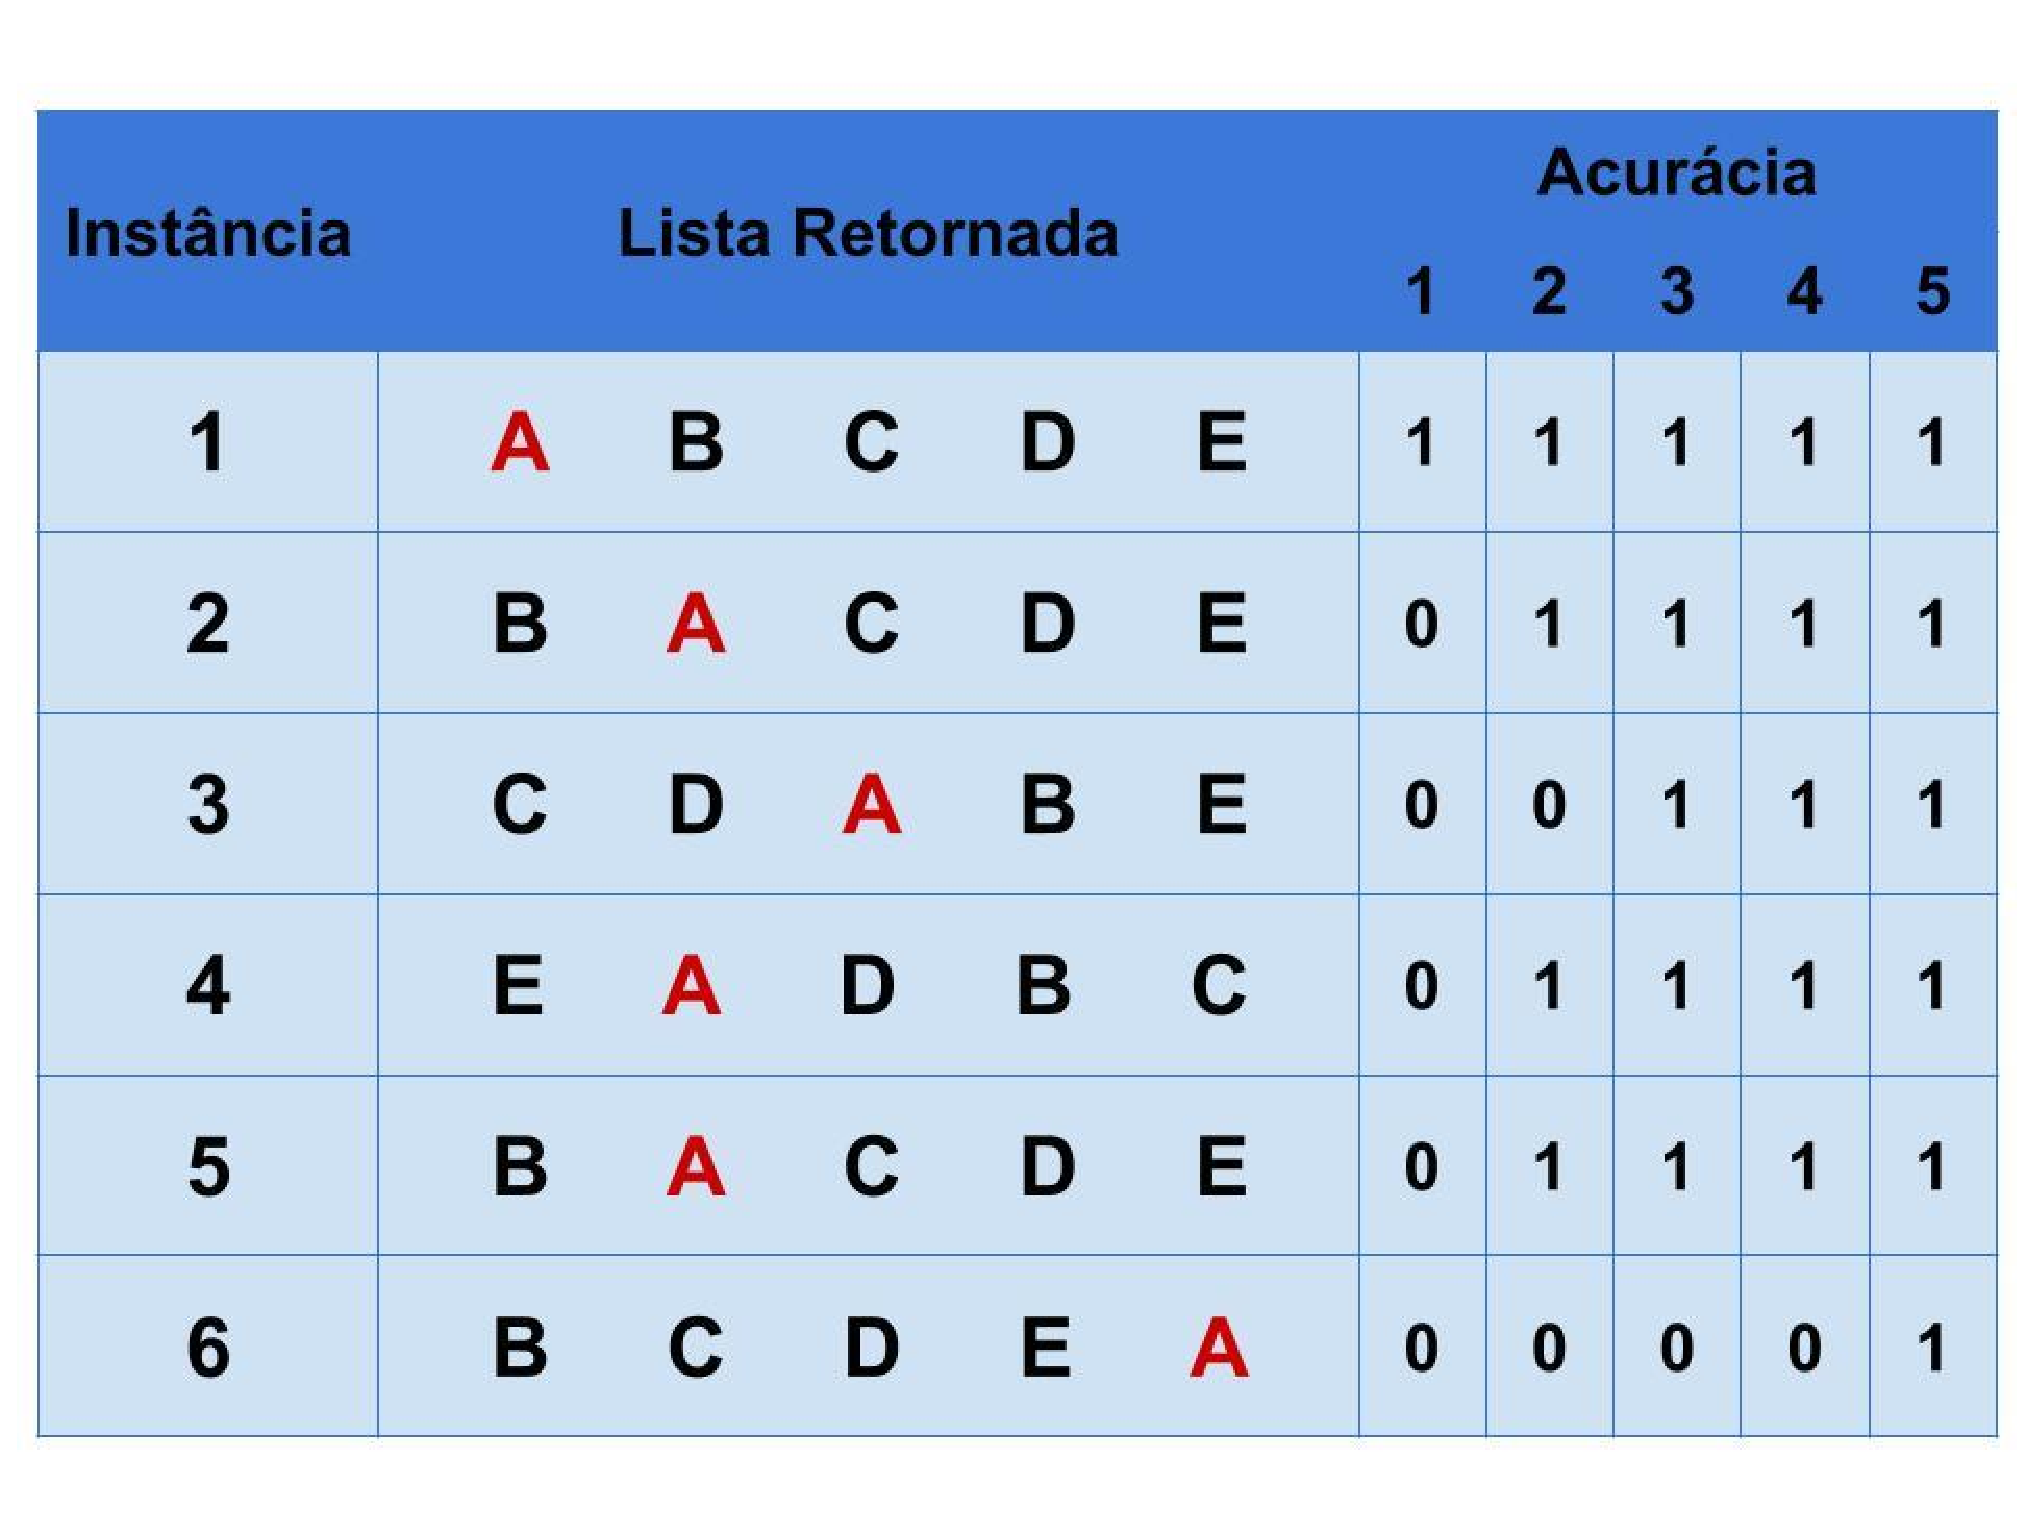
\includegraphics[width=100mm,scale=0.7]{images/descricaodostestes01.eps}
  \caption{Exemplos de listas e suas acurácias.}
  \label{fig:descricaodostestes01}
\end{figure}

Existe ainda uma diferença no cálculo da \textit{k-Acurácia} para o \textit{benckmark} dos testes.
Como a lista de \textit{benckmark} é construída a partir de uma distribuição de probabilidades, podem ocorrer empates.
Quando a probabilidade da classe verdadeira está empatada com a de uma ou mais classes, múltiplas listas poderiam ser criadas a partir desta distribuição.
Considere o caso onde temos as classes A, B e C com probabilidades 0.4, 0.4 e 0.2 respectivamente e a classe verdadeira é A.
Com essas probabilidades podemos ter as listas de saída (1) A, B e C ou (2) B, A e C.
No primeiro caso temos as acurácias de um a três iguais a um.
No segundo caso temos a \textit{1-Acurácia} igual a zero e o restante igual a um.
Entretanto, por ter acesso às probabilidades, a métrica divide os valores.
Teremos então \textit{1-Acurácia} igual 0.5, \textit{2-Acurácia} igual a 0.5 e \textit{3-Acurácia} igual a 1.

Note que todos os cálculos citados até agora são feitos por instância. 
Ao gerar listas de saída para múltiplas instâncias, os valores obtidos para cada acurácia são somados, formando um valor total por \textit{i-Aurácia}.
Este valor total é então dividido pelo número de instâncias que foram ranqueadas e multiplicado por cem.
Com isso os valores das acurácias apresentados neste trabalho estão na forma de percentuais.

Desta forma, podemos calcular os valores percentuais das acurácias ao longo de todos os exemplos da figura \ref{fig:descricaodostestes01}.
Os valores são apresentados na tabela \ref{tab:valoresacuraciasexemplo}.

\begin{table}[h!]
  \begin{center}
    \begin{tabular}{cc}
      \hline
      \textbf{Acurácia} & \textbf{Valor Percentual} \\
      \hline

      1 & 16,67 \% \\
      2 & 66,67 \% \\
      3 & 83,33 \% \\
      4 & 83,33 \% \\
      5 & 100 \% \\

      \hline
    \end{tabular}
    \caption{Valores percentuais das acurácias do exemplo}
    \label{tab:valoresacuraciasexemplo}
  \end{center}
\end{table}

\section{Resultados dos Testes}

Todos os testes realizados neste capítulo foram realizados com validação cruzada com partição em dez grupos.
Novamente, os componentes do \textit{framework} Weka foram utilizados para realizar as validações.
Além disso, ao executar o programa 10 GB de memória são reservados para o \textit{heap} da Máquina Virtual Java com o comando \textit{java -Xmx10g}.

Todos os testes foram executados em máquinas virtuais no ambiente \textit{Google Cloud Platform}. 
Estas máquinas tinham a seguinte configuração: sistema operacional Linux Ubuntu 14.04, duas unidades de processamento (vCPU) e 13 GB de memória RAM.

Na Tabela \ref{tab:algoritmostestes} são apresentadas as configurações de algoritmos usados nos testes. Todas as classes utilizadas são do pacote \textit{weka.classifiers}.

\begin{table}[h!]
  \begin{center}
    \begin{tabular}{ccc}
      \hline
      \textbf{Algoritmo} & \textbf{Classe Weka} & \textbf{Opções} \\
      \hline

      Árvore de Decisão & trees.J48 & padrão \\
      Naive Bayes & bayes.NaiveBayes & padrão \\
      Support Vector Machine (SVM) & functions.SMO & padrão \\
      Random Forest & trees.RandomForest & padrão \\
      k vizinhos mais próximos (KNN) & lazy.IBk & K = 5, 7 e 9 \\

      \hline
    \end{tabular}
    \caption{Configurações dos algoritmos}
    \label{tab:algoritmostestes}
  \end{center}
\end{table}

Na Tabela \ref{tab:datasets} são apresentados as características gerais dos conjuntos de dados utilizados nos testes.
A maioria dos conjuntos de dados foi retirado do repositório \textit{UCI Machine Learning Repository}, disponível na internet no endereço http://archive.ics.uci.edu/ml/.
Além disso, em alguns casos o conjunto de dados foi pré-processado e reduzido para facilitar a realização dos diversos testes.
A exceção é o conjunto de dados Data-Zero, este não foi retirado do mesmo repositório.
O conjunto de dados Data-Zero representa a ocorrência de falhas em uma rede com diversos nódos.
Seu atriburo classe denota em qual nódo a falha ocorreu.

\begin{table}[h!]
  \begin{center}
    \begin{tabular}{cccc}
      \hline
      \textbf{Conjunto de Dados} & \textbf{Instâncias} & \textbf{Atributos} & \textbf{Valores de Classe} \\
      \hline

      Iris & 150 & 5 & 3 \\
      Wine & 178 & 14 & 3 \\ 
      Glass & 214 & 10 & 7 \\
      Balance-Scale & 625 & 5 & 3 \\
      Segment-Challenge & 1500 & 20 & 7 \\
      Car & 1728 & 7 & 4 \\
      Data-Zero & 2846 & 202 & 42 \\
      Nursery & 3330 & 9 & 5 \\
      Poker-Hand & 3712 & 11 & 10 \\      
      Covtype-01percent & 5810 & 55 & 7 \\
      Covtype-10percent & 58101 & 55 & 7 \\    

      \hline
    \end{tabular}
    \caption{Conjuntos de dados}
    \label{tab:datasets}
  \end{center}
\end{table}

\subsection{Análise dos Tempos de Execução}

A Tabela \ref{tab:tempostestes} ilustra os tempos médios de execução para o conjunto de dados \textit{segment-challenge}, com uma lista de saída com tamanho três e validação cruzada com partição em dez grupos.
Os resultados para os demais conjuntos de treino seguem a mesma tendência e podem ser vistos por completo no apêndice.

A coluna \textit{Configuração} indica como a lista de saída foi construída.
Isto é, o teste pode ter empregado o modelo gerado pelo \textit{classificador} diretamente para construir a lista ou uma versão do método proposto (\textit{estática} ou \textit{dinâmica}).
A coluna \textit{Treino} informa o tempo médio de treinamento do modelo e a coluna \textit{Teste} o tempo médio que o modelo levou para gerar as listas de saída para as instâncias.
Estes valores foram obtidos com a média aritimética de cada Tempo ao longo das iterações da validação cruzada.


Note que, para todos os casos, temos que o tempo total do classificador é menor que os tempos das versões do método proposto.
Este resultado já era esperado, visto que o método proposto precisa treinar diversos classificadores para construir a lista de saída.
Além disso, a versão estática apresentou tempos totais maiores que a dinâmca.
Isso ocorre pois a primeira precisa treinar todos os classificadores possíveis a partir do conjunto de treino, enquanto a segunda treina apenas aqueles que são efetivamente utilizados.
Lembre que a versão dinâmica treina o modelo ao mesmo tempo que classifica as instâncias, portanto não é possível separar os tempos de treino e teste.
Por fim, uma vez que ambas as versões do método incorrem o mesmo resultado, somente a versão dinâmica foi utilizada nos demais testes apresentados neste capítulo.

\begin{table}[h!]
  \begin{center}
    \begin{tabular}{ccccc}
      \hline
      \textbf{Algoritmo} & \textbf{Configuração} & \textbf{Treino (ms)} & \textbf{Teste (ms)} & \textbf{Total (ms)}\\
      \hline

      Árvore de Decisão & classificador & 91.85 & 7.89 & 99.74\\
      Árvore de Decisão & estática & 515.80 & 6.70 & 522.51\\
      Árvore de Decisão & dinâmica & - & 405.87 & 405.87\\
      Naive Bayes &  classificador & 11.42 & 38.26 & 49.68\\
      Naive Bayes &  estática & 99.01 & 40.43 & 139.44\\
      Naive Bayes &  dinâmica & - & 100.95 & 100.95\\
      SVM & classificador & 240.37 & 4.18 & 244.55\\
      SVM & estática & 1646.29 & 6.45 & 1652.74\\
      SVM & dinâmica & - & 1340.57 & 1340.57\\
      Random Forest &  classificador & 449.76 & 8.62 & 458.38\\
      Random Forest &  estática & 5686.47 & 14.43 & 5700.89\\
      Random Forest &  dinâmica & - & 3934.28 & 3934.28\\
      KNN 5 & classificador & 0.89 & 23.76 & 24.66\\
      KNN 5 & estática  & 90.49 & 111.69  & 202.19\\
      KNN 5 & dinâmica  & - & 101.84 & 101.84\\


      \hline
    \end{tabular}
    \caption{Tempos médios de execução em milisegundos}
    \label{tab:tempostestes}
  \end{center}
\end{table}

\subsection{Análise das Acurácias}

A Tabela \ref{tab:acuracias} exibe os valores de acurácia médios para cada algoritmo. 
Estes valores foram obtidos com a média aritimética de cada acurácia ao longo de todos os conjuntos de dados testados.
Novamente, a coluna \textit{Configuração} indica a forma que a lista de saída foi gerada. 
O valor \textit{classificador} significa que nestes testes usamos a distribuição de probabilidades do classificador para gerar a lista de saída, ou seja, é o \textit{benckmark} daquele teste.
Já o valor \textit{metaclassificador} significa que o método proposto (versão dinâmica) foi utilizado.
No intuito de facilitar a comparação, apresentamos as acurácias 1, 2 e 3 do classificador e do metaclassificador sempre em linhas subsequentes.

Além disso, é possivel observar de forma rápida na tabela \ref{tab:acuracias2} quantas vezes cada configuração obteve o melhor resultado em cada acurácia.
Note que a contagem da tabela \ref{tab:acuracias2} se refere aos testes individuais e não às médias, ou seja, um teste por combinação de algoritmo e conjunto de dados.


\begin{table}[h!]
  \begin{center}
    \begin{tabular}{ccccc}
      \hline
      \textbf{Algoritmo} & \textbf{Configuração} & \textbf{1-Acurácia} & \textbf{2-Acurácia} & \textbf{3-Acurácia}\\
      \hline

      Árvore de Decisão & classificador & 75.61 & 82.26 & 84.88\\
      Árvore de Decisão & metaclassificador & 75.69 & 87.63 & 92.78\\
      Naive Bayes & classificador & 66.72 & 78.92 & 86.3\\
      Naive Bayes & metaclassificador & 66.72 & 78.93 & 86.3\\
      Random Forest & classificador & 82.62 & 91.15 & 95.12\\
      Random Forest & metaclassificador & 82.63 & 90.96 & 95.25\\
      SVM & classificador & 72.71 & 84.22 & 89.58\\
      SVM & metaclassificador & 72.71 & 84.08 & 89.92\\
      KNN 5 & classificador & 75.85 & 86.11 & 90.06\\
      KNN 5 & metaclassificador & 75.85 & 86.01 & 91.05\\
      KNN 7 & classificador & 74.79 & 85.69 & 89.75\\
      KNN 7 & metaclassificador & 74.62 & 85.4 & 90.43\\
      KNN 9 & classificador & 74.07 & 85.45 & 89.93\\
      KNN 9 & metaclassificador & 74.02 & 84.41 & 89.85\\


      \hline
    \end{tabular}
    \caption{Valores de acurácia médios por algorítimo}
    \label{tab:acuracias}
  \end{center}
\end{table}

\begin{table}[h!]
  \begin{center}
    \begin{tabular}{cccc}
      \hline
      \textbf{Ganhador} & \textbf{1-Acurácia} & \textbf{2-Acurácia} & \textbf{3-Acurácia}\\
      \hline

      Classificador & 20 & 16 & 13\\
      Metaclassificador & 20 & 34 & 29\\
      Empate & 30 & 20 & 28\\

      \hline
    \end{tabular}
    \caption{Número de vezes que cada configuração ganhou}
    \label{tab:acuracias2}
  \end{center}
\end{table}

Observe na Tabela \ref{tab:acuracias} que os valores da \textit{1-Acurácia} são sempre muito similares para o classificador e o metaclassifficador.
Este resultado é esperado pois o primeiro modelo interno do metaclassificador (aquele que foi treinado com todo o conjunto de treino) é sempre igual ao modelo que gera a distribuição de probabilidades para o \textit{benckmark}.
Como foi explicado, quando ocorre empate de probabilidades na construção desse \textit{benckmark}, a métrica \textit{k-Acurácia} distribui o valor total entre as posições empatadas.
Desta forma, as diferenças na \textit{1-Acurácia} observadas na Tabela \ref{tab:acuracias} são devidas ao tratamento diferente nestes casos de empate.

Ainda na Tabela \ref{tab:acuracias}, note que o metaclassificador destacou-se nos testes com o algoritmo Árvore de Decisão.
Ele teve cerca de 5\% de vantagem na \textit{2-Acurácia} e 8\% na \textit{3-Acurácia}.
Nos demais casos as diferenças nas acurácias foram muito pequenas, em alguns o classificador teve um resultado marginalmente melhor em outros o metaclassificador.